\documentclass[12pt]{article}
\setlength\parindent{0pt}
\usepackage{fullpage}
\usepackage[margin=0.5in]{geometry}
\usepackage{amsmath}
\usepackage{graphicx}
\setlength{\parskip}{1.5em}
\def\LL{\left\langle}   % left angle bracket
\def\RR{\right\rangle}  % right angle bracket
\def\LP{\left(}         % left parenthesis
\def\RP{\right)}        % right parenthesis
\def\LB{\left\{}        % left curly bracket
\def\RB{\right\}}       % right curly bracket
\def\PAR#1#2{ {{\partial #1}\over{\partial #2}} }
\def\PARTWO#1#2{ {{\partial^2 #1}\over{\partial #2}^2} }
\def\PARTWOMIX#1#2#3{ {{\partial^2 #1}\over{\partial #2 \partial #3}} }
\newcommand{\BI}{\begin{itemize}}
\newcommand{\EI}{\end{itemize}}
\newcommand{\BE}{\begin{displaymath}}
\newcommand{\EE}{\end{displaymath}}
\newcommand{\BNE}{\begin{equation}}
\newcommand{\ENE}{\end{equation}}
\newcommand{\BEA}{\begin{eqnarray}}
\newcommand{\EEA}{\nonumber\end{eqnarray}}
\newcommand{\EL}{\nonumber\\}
\newcommand{\la}[1]{\label{#1}}
\newcommand{\ie}{{\em i.e.\ }}
\newcommand{\eg}{{\em e.\,g.\ }}
\newcommand{\cf}{cf.\ }
\newcommand{\etc}{etc.\ }
\newcommand{\Tr}{{\rm tr}}
\newcommand{\etal}{{\it et al.}}
\newcommand{\OL}[1]{\overline{#1}\ } % overline
\newcommand{\OLL}[1]{\overline{\overline{#1}}\ } % double overline
\newcommand{\OON}{\frac{1}{N}} % "one over N"
\newcommand{\OOX}[1]{\frac{1}{#1}} % "one over X"

\begin{document}

\begin{center}
	\Large \sc Homework 9
	
	\normalsize Due Wednesday, May 4
\end{center}
\pagenumbering{gobble}

\begin{enumerate}
	  \item Rotational motion introduces many new terms, and in order to make sense of conversations about rotation, you should be familiar with them. In your own words and using
	{\it no mathematics}, define the following and give the dimensions of each of the following:
	
	\begin{enumerate}
		\item Angular velocity
		\item Angular acceleration
		\item Tangential velocity
		\item Radial acceleration
		\item Tangential acceleration
		\item Torque
		\item Angular momentum
		
	\end{enumerate}
	\bigskip
	\bigskip
	
	\item  The CD-ROM drive in a computer accelerates a disk from rest to its full speed of 20000 revolutions per minute; it does so uniformly over 5 seconds. The disk is 6 cm in radius.
	
	\begin{enumerate}
		\item Is it correct to write $\alpha = 4000~{\rm rev} \cdot {\rm min}^{-1} \cdot {\rm s}^{-1}$? Explain.
		
		\item What is the maximum angular velocity in our conventional units of radians per second?
		
		\item What is its angular acceleration?
		
		\item How many times does it spin during this interval?
		
		\item After four seconds, what is the {\it tangential velocity} of a point along the edge of the disk?
		
		\item After four seconds, what is the {\it angular velocity} of a point along the edge of the disk?
		
		\item After four seconds, how many times has the disc rotated?
		
%		\item After four seconds, what is the {\it tangential acceleration} of a point along the edge? 
%		
%		\item After four seconds, what is the {\it radial acceleration} of a point along the edge? Speculate on the engineering consequences of this figure; how large is it compared to other accelerations you know?
	\end{enumerate}

	\bigskip
	\bigskip
	
	\item Suppose that you want to hold a meter stick horizontal to the ground by touching it
	with only two fingers. One finger is at the 10 cm mark, while the other finger is at the
	20 cm mark. The meter stick has a weight of 1 N. What must you do with your fingers,
	and what normal forces do they exert on the meter stick?
	What if your fingers are at the 10 cm and 12 cm marks?
	
	If you are having trouble
	with this problem, go get a meter stick and physically play with it. We will put a meter stick in the Physics Clinic for people to play with.
	\bigskip
	\bigskip
	\newpage
	
	 \item A construction worker takes a break for lunch, resting on a steel beam.
	
	\begin{minipage}{0.5\textwidth}
		The steel
		beam has a mass of 1450 kg, and the construc-
		tion worker shown has a mass of 80 kg. They sit
		3.2 meters from the end of the beam. The cable is rated to transmit a tension of 15 kN.
	\end{minipage}
	\begin{minipage}{0.5\textwidth}
		\begin{center}
			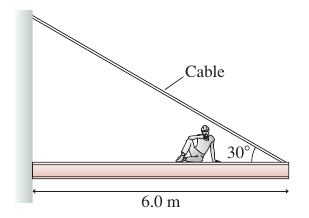
\includegraphics[width=0.7\textwidth]{person-on-girder.png}
		\end{center}
	\end{minipage}
	
	Should they be worried that the cable might fail?
	
	\bigskip
	\bigskip
	\item A castle's drawbridge consists of a heavy wooden plank that can be opened or closed using a rope, as shown below:
	
	\begin{minipage}{0.5\textwidth}
		The rope is attached to the door 4/5 of the way down its length; the left side of the plank is attached to a hinge
		in the ground.
		The bridge is left in a partially-raised state by a careless sentry. It makes an angle of $30^\circ$ with the horizontal; the rope that supports it is perpendicular to the
		bridge.
	\end{minipage}
	\begin{minipage}{0.5\textwidth}
		\begin{center}
			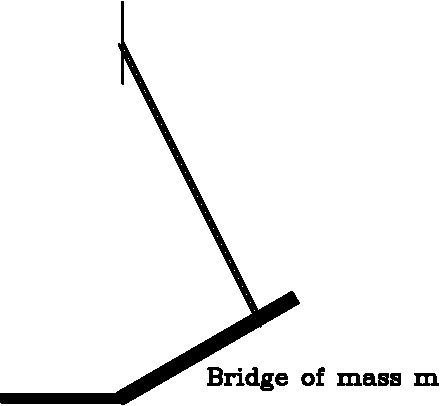
\includegraphics[width=0.6\textwidth]{door-crop.pdf}
		\end{center}
		
	\end{minipage}
	\medskip
	
	If the mass of the door is $m$, calculate the tension $T$ in the rope in terms of $\theta$, $m$, and $g$.
	
		\bigskip
	
	\bigskip
	
\item A person rolls a basketball ($I=\frac{2}{3}mr^2$) down a slope; the slope is inclined at an angle $\theta=15^\circ$. The basketball rolls without slipping down the slope.

At the same time, another person slides a piece of ice down the slope. There {\it is} friction between the ice and the slope -- just not very much.

What must the coefficient of kinetic friction $\mu_k$ between the ice and the slope be such that the piece of ice and the basketball have the same speed when they reach the bottom?

\bigskip
\bigskip
\newpage

\item A ``merry-go-round'' is a large horizontal platform for children to play on that can rotate freely. 

\begin{minipage}{0.5\textwidth}
Imagine a certain merry-go-round has a radius of $r=3$ m and a mass of 200 kg, and has been constructed out of fancy and well-lubricated bearings so that it rotates freely without friction.
\bigskip


Suppose a child of mass 40 kg runs and jumps on the edge of the platform at 5 m/s; when they land on the edge, they are moving tangent to it. (See the diagram.)
\end{minipage}
\begin{minipage}{0.5\textwidth}
	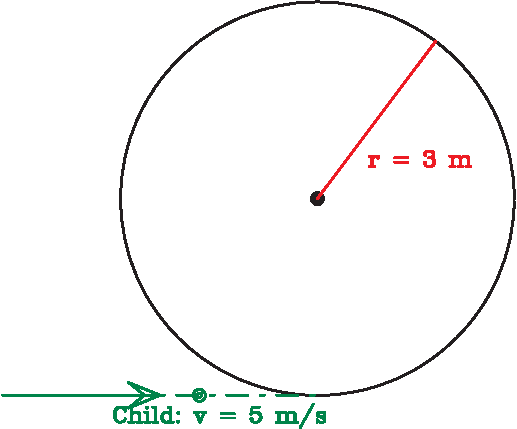
\includegraphics[width=0.7\textwidth]{mgr-crop.pdf}
\end{minipage}

	\begin{enumerate}
		\item Once the child jumps on the platform, how will it move?
		\item Now, imagine that the child walks to the center of the platform. How will it be moving now?
	\end{enumerate}

\bigskip\bigskip

\item An large old iron wheel of mass $m$, still connected to its axle, has been abandoned by a roadside. A person wants to move it, so they tie a rope to the axle, set the wheel up on its edge, and pull horizontally with a tension $T$. The coefficient of static friction between the wheel and the ground is $\mu_s$ and the coefficient of kinetic friction is $\mu_k$.

They pull gently enough that the wheel rolls without slipping.

\begin{enumerate}
	\item Determine, in terms of $m$, $T$, $g$, and $\mu$, the acceleration of the wheel. (Your result may not depend on all of these.)
	
	\item Determine, in terms of $m$, $T$, $g$, and $\mu$, the frictional force between the wheel and the ground. (Your result may not depend on all of these.)	
\end{enumerate}

\newpage
%
%\item {\it (This problem is worth ten points extra credit if you complete it fully.)}
%
%A cylinder ($I=\frac{1}{2}mr^2$) rolls without slipping down an inclined plane of length $L$, angled at an angle $\theta$ to the horizontal. The
%coefficient of static friction between them is $\mu_s=0.5$.
%
%\begin{enumerate}
%	
%	\item Draw a (large) extended force diagram for the cylinder. Consider carefully in which direction the frictional force at the point of contact points.
%	\item Is the frictional force equal to $\mu_s F_N$, or some other value that depends on the angle $\theta$? Explain, thinking about what happens as $\theta \rightarrow 0$.
%	(If the frictional force is not equal to $\mu_s F_N$, just use $F_f$ to represent it in equations.)
%	\item The ordinary ``translational'' work-energy theorem says that a force $\vec F$ acting over a displacement $\vec d$ causes a change in translational kinetic energy:
%	$\Delta (\frac{1}{2}mv^2) = \vec F \cdot \vec d$.
%	Find the ``translational work'' done by the gravitational force and by the frictional force.
%	\item The ``rotational'' work-energy theorem says that a torque $\tau $ acting over an object rotating through an angle $\Delta \theta$ causes a change in rotational kinetic energy: $\Delta (\frac{1}{2}I\omega^2) = \tau \Delta \theta$.
%	Find the ``rotational work'' done by the gravitational force and by the frictional force.
%	\item If we consider ``translational kinetic energy'' $\frac{1}{2}mv^2$ and ``rotational kinetic energy'' $\frac{1}{2}I\omega^2$ as the same thing, what is the total
%	work (rotational plus translational) done by the frictional force?
%	\item Is it accurate to say that the frictional force here converts translational kinetic energy into rotational kinetic energy? Explain.
%	\item Comment on the validity of using energy methods to solve problems like (2). Do you need to worry about the frictional forces when considering translational
%	and rotational kinetic energy together?
%	\item By any method you like, calculate the size of the frictional force $F_f$. (There are two ways to do this. One involves energy methods; the other involves
%	examining the force diagram and thinking about the relation between $a$ and $\alpha$.)
%\end{enumerate}
 


\end{enumerate}



\end{document}